\documentclass[a4paper,11pt]{article}
\usepackage{amsmath,amssymb,amsthm, tikz,titlesec,hyperref,esint,braket, graphicx}
\usepackage[a4paper,margin=2cm]{geometry}
\linespread{1.3}
\newtheorem{claim}{Claim}[section]

\newcommand\name{Park Chanwoo}   % Name of the student
\newcommand\university{KAIST} % Name of the university
\newcommand\department{Physics} % Name of the department
\newcommand\studentid{20230297} % Student ID
\newcommand\s{\,\;}


\newenvironment{solution}[1]
  {\renewcommand\qedsymbol{$\square$}\begin{proof}[\textbf{Solution#1}]}
  {\end{proof}}
\newenvironment{note}
  {\renewcommand\qedsymbol{$\blacksquare$}\begin{proof}[\textnormal{\textbf{note}}]}
  {\end{proof}}

\title{KAIST\\2025 PH475 Quantum Information I\\
Homework 1\bigskip}
\author{\textbf{\Large \name} \\
% University: \university\\
Department: \department\\
Student ID: \studentid}
\date{\today}

\begin{document}
\thispagestyle{empty}
\maketitle
\tableofcontents
\titleformat{\section}[frame]{\pagebreak}{\filright
\footnotesize  \enspace \textsf{KAIST --- PH475 Quantum Information I 2025 Spring}\enspace}{6pt}{\Large\bfseries\filcenter}

\newcommand{\der}[2][]{\frac{d #1}{d #2}}
\newcommand{\pder}[2][]{\frac{\partial #1}{\partial #2}}
\newcommand{\grad}{\operatorname{grad}}
\newcommand{\diver}{\operatorname{div}}
\newcommand{\curl}{\operatorname{curl}}



\section{\#1}

\begin{solution}{}
    The Hadamard gate is given by
    \begin{equation}
        H = \ket{+}\bra{0}+\ket{-}\bra{1}
    \end{equation}
    
    (a)
    The $\pm$ states are given by
    \begin{equation}
        \ket{+} = \frac{1}{\sqrt2}\ket{0} + \frac{1}{\sqrt2}\ket{1}, \quad
        \ket{=} = \frac{1}{\sqrt2}\ket{0} - \frac{1}{\sqrt2}\ket{1}
    \end{equation}
    
    Hence, the Hadamard gate in computational basis is
    \begin{equation}
        H=\frac{1}{\sqrt2}\ket{0}\bra{0} + \frac{1}{\sqrt2}\ket{1}\bra{0} + \frac{1}{\sqrt2}\ket{0}\bra{1} - \frac{1}{\sqrt2}\ket{1}\bra{1}
    \end{equation}
    
    (a) The adjoint is
    \begin{align}
        H^\dagger&=\left(\frac{1}{\sqrt2}\right)^*\ket{0}\bra{0} + \left(\frac{1}{\sqrt2}\right)^*\ket{0}\bra{1} + \left(\frac{1}{\sqrt2}\right)^*\ket{1}\bra{0} + \left(-\frac{1}{\sqrt2}\right)^*\ket{1}\bra{1} \\
        &=\frac{1}{\sqrt2}\ket{0}\bra{0} + \frac{1}{\sqrt2}\ket{1}\bra{0} + \frac{1}{\sqrt2}\ket{0}\bra{1} - \frac{1}{\sqrt2}\ket{1}\bra{1} \\
        &=H
    \end{align}

    (b)
    \begin{align}
        H^2&=H^\dagger H\\
        &=\left(\ket{0}\bra{+}+\ket{1}\bra{-}\right)\left(\ket{+}\bra{0}+\ket{-}\bra{1}\right)\\
        &=\ket{0}\braket{+|+}\bra{0} + \ket{0}\braket{+|-}\bra{1} + \ket{1}\braket{-|+}\bra{0} + \ket{1}\braket{-|-}\bra{1}\\
        &=\ket{0}\bra{0} + \ket{1}\bra{1} = I
    \end{align}

    (c) Try the ansatz
    \begin{equation}
        \ket{\psi} = \cos\theta\ket{0} + \sin\theta\ket{1}
    \end{equation}

    \begin{align}
        H\ket\psi &= \frac{1}{\sqrt2}\left[\cos\theta + \sin\theta\right]\ket{0} + \frac{1}{\sqrt2}\left[\cos\theta - \sin\theta\right]\ket{1} \\
        &= \cos\left(\frac{\pi}{4} - \theta\right)\ket{0} + \sin\left(\frac{\pi}{4} - \theta\right)\ket{0}
    \end{align}

    if $\pi/4 - \theta = \theta$ then $H\ket\psi = \ket\psi$

    Hence, 
    \begin{equation}
        \ket{H=1} = \cos(\pi/8)\ket{0} + \sin(\pi/8)\ket{1}
    \end{equation}

    Since $\sin(x + \pi) = \sin x$ and $\cos(x + \pi) = \cos x$, $\pi/4 - \theta = \theta + \pi$ also gives a eigenvector associated with eigenvalue $-1$. 
    \begin{align}
        \ket{H=-1} &= \cos(-3\pi/8)\ket{0} + \sin(-3\pi/8)\ket{1} \\
         &= \sin(\pi/8)\ket{0} - \cos(\pi/8)\ket{1} 
    \end{align}

    Here the sine and cosine values are:
    \begin{gather*}
        \cos\frac{\pi}{8} = \frac{\sqrt{2 + \sqrt{2}}}{2}\\
        \sin\frac{\pi}{8} = \frac{\sqrt{2 - \sqrt{2}}}{2}
    \end{gather*}
\end{solution}

\section{\#2}

\begin{solution}{}
    (1)
    \begin{figure}[h!]
        \centering
        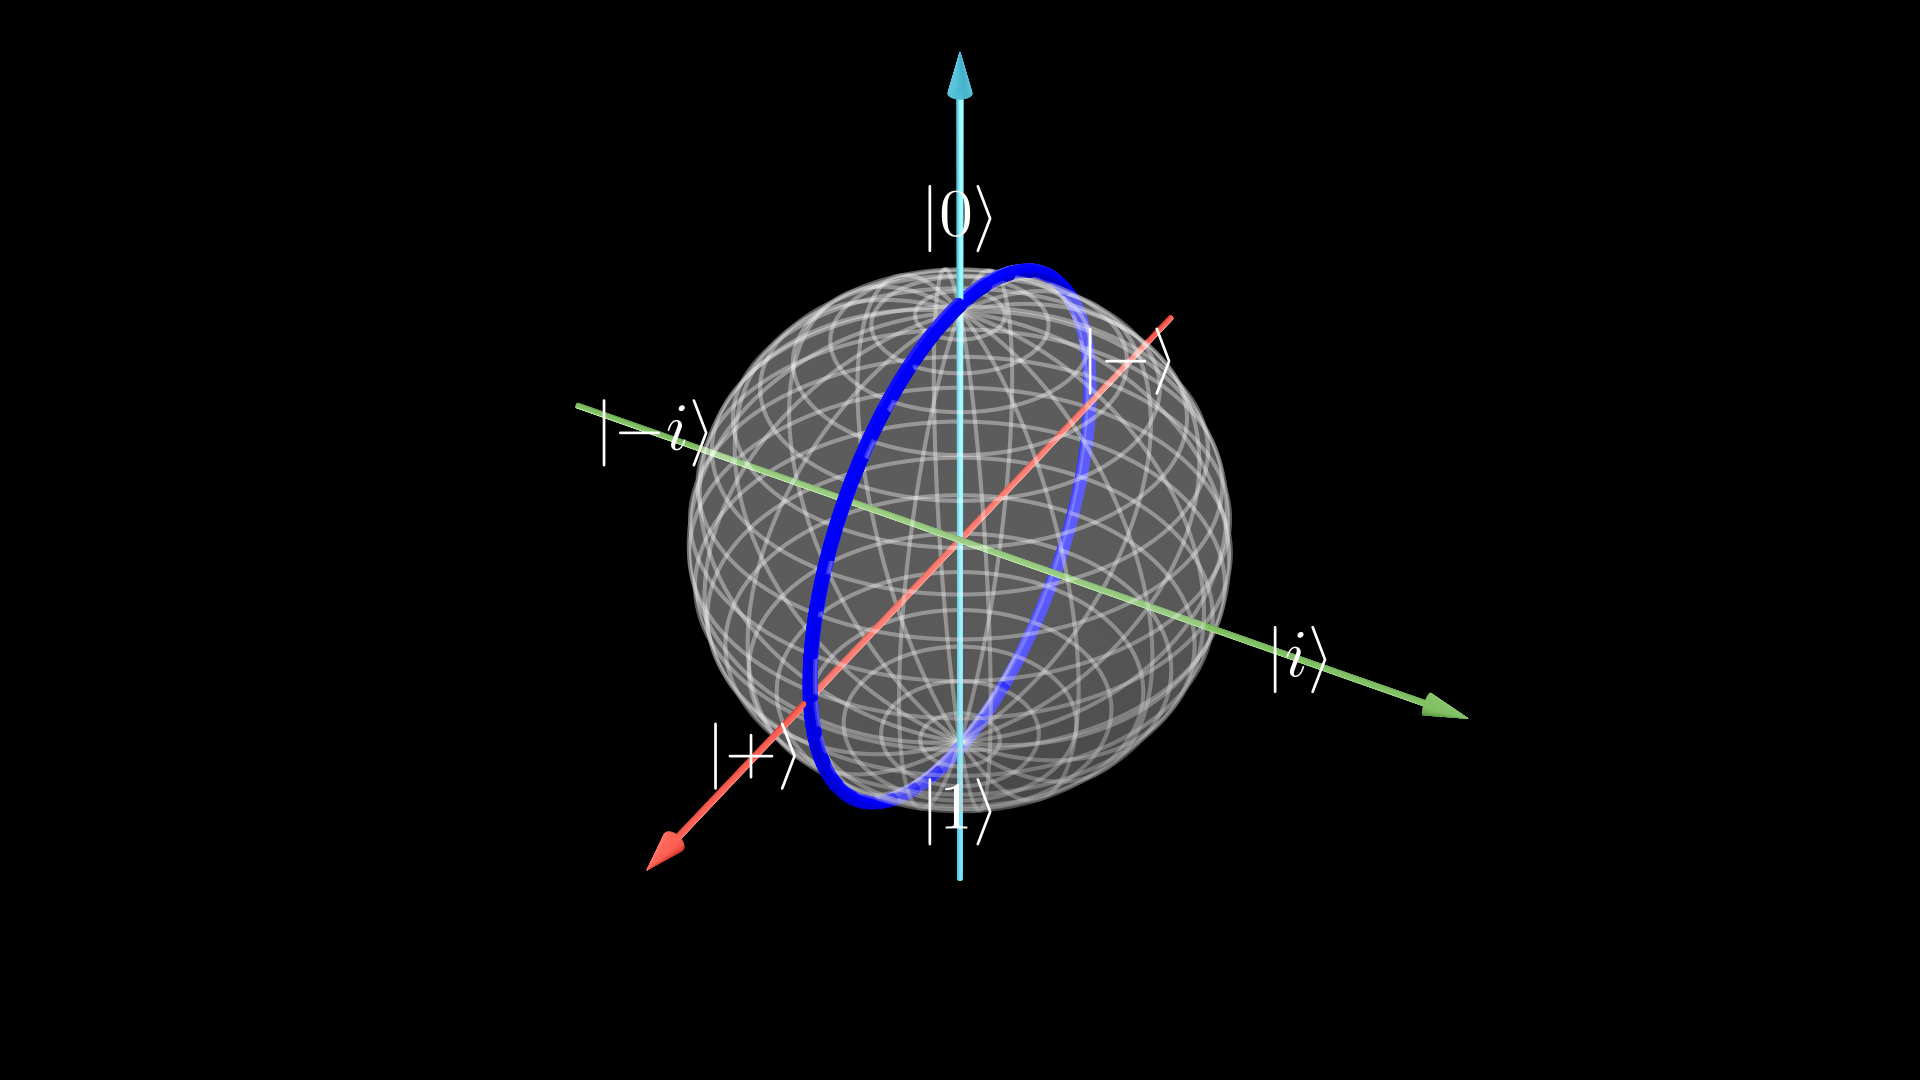
\includegraphics[width=0.5\linewidth]{ExampleSphere_ManimCE_v0.19.0.png}
        \caption{The trajectory of $\ket\psi$ on Bloch sphere}
        \label{fig:bloch}
    \end{figure}
    
    (2) The expectation value of the Pauli z operator is
    \begin{align}
        \braket{Z} &= (+1)|\braket{0|\psi}|^2 + (-1)|\braket{1|\psi}|^2\\
        &=\cos^2(\theta/2) - \sin^2(\theta/2) \\
        &=\cos\theta
    \end{align}

    (3) and the variance is
    \begin{align}
        \braket{Z^2} - \braket{Z}^2&= (+1)^2|\braket{0|\psi}|^2 + (-1)^2|\braket{1|\psi}|^2 - \cos^2\theta\\
        &=\cos^2(\theta/2) + \sin^2(\theta/2) - \cos^2\theta\\
        &=\sin^2\theta
    \end{align}

    (4) At $\theta = 0$ and $\theta = \pi$, The variance is minimized. At those points,  the state is exactly $\ket{0}$ or $\ket{1}$. At $\theta = \frac{\pi}{2}$, The variance is maximized. It is equal superposition of $\ket{0}$ and $\ket{1}$
    
    
\end{solution}

\end{document}
